\documentclass[conference]{IEEEtran}
\IEEEoverridecommandlockouts
\usepackage{cite}
\usepackage{amsmath,amssymb}
\usepackage{graphicx}
\usepackage{booktabs}
\usepackage{xcolor}
\usepackage{url}
\usepackage{tikz}
\usetikzlibrary{arrows.meta,positioning}
\usepackage{algorithm}
\usepackage{algpseudocode}
\usepackage{placeins}

\begin{document}

\title{AI-Based Predictive Traffic Signal Control for Alternative Roads During Unexpected Incidents}

\author{\IEEEauthorblockN{Atheer Bahussein}
\IEEEauthorblockA{\textit{Department of CSIT} \\ \textit{Jeddah International College}\\ Jeddah, Saudi Arabia \\ 251200499@jicollege.edu.sa}
\and
\IEEEauthorblockN{Mnar Alnaghes}
\IEEEauthorblockA{\textit{Department of CSIT} \\ \textit{Jeddah International College}\\ Jeddah, Saudi Arabia \\ m.alnaghes@jicollege.edu.sa}}

\maketitle

\begin{abstract}
Unexpected incidents push diverted traffic onto alternative roads faster than reactive signal control can respond. We design a closed loop that couples camera-based incident detection (YOLO with ByteTrack) with an incident-conditioned graph forecaster and a predictive max-pressure signal controller with a spillback guard, and we evaluate the forecasting and control stages in SUMO with detection latency and misses emulated in the loop. On a $4\times4$ grid with an arterial corridor, using an incident location unseen in training and 8 random seeds per scenario, a gradient-boosted forecaster reduced 2-minute queue-forecast error near the incident by 16\% relative to persistence. This did not translate into better control: the predictive controller stayed within 1.2\,s/veh of reactive max-pressure in all four scenarios, and SUMO's actuated controller achieved the lowest delay throughout (14--16\% below max-pressure under full closure). No controller shifted queuing to links away from the incident. With unseen incident durations, the predictive controller was equal or worse, and the forecaster did not generalise to longer incidents. We explain why short-horizon forecasts add little to a pressure policy that reacts every second, and identify conditions under which prediction is more likely to pay off.
\end{abstract}

\begin{IEEEkeywords}
smart mobility, incident detection, YOLO, graph forecasting, max-pressure, traffic signal control, SUMO
\end{IEEEkeywords}

\section{Introduction}
Urban road networks operate close to capacity during peak hours, so even a short loss of capacity can have network-wide effects. Congestion is commonly divided into \emph{recurrent} congestion, which follows predictable daily patterns, and \emph{non-recurrent} congestion caused by crashes, breakdowns, lane closures and other unexpected events. Signal plans and most adaptive systems are designed and tuned for recurrent demand. Incidents break these patterns: a blocked lane suddenly removes capacity, queues grow behind it, and drivers start to divert to parallel and crossing streets within minutes.

The diverted traffic creates a second problem on the \emph{alternative roads}. Their signal timings were not planned for the extra demand, so queues build up at intersections that were uncongested shortly before. When these queues reach the upstream intersection they block it (spillback), and a local incident can turn into gridlock across several blocks. The damage therefore depends not only on the incident itself but on how quickly the signals on the diversion routes adapt.

Deployed adaptive systems such as SCOOT~\cite{robertson1991scoot} and SCATS~\cite{sims1980scats}, and most reinforcement learning (RL) controllers~\cite{genders2016deep,wei2018intellilight}, are \emph{reactive}: they change timings after detectors measure longer queues or higher occupancy. By the time the measurements show the problem, the queue may already be close to spilling back. RL controllers face an additional risk, because an incident shifts both demand and driver behaviour away from the conditions they were trained on~\cite{nguyen2025trex}.

Smart-city infrastructure offers a way to act earlier. Roadside cameras can detect a stopped vehicle within seconds, and graph-based models can forecast how congestion spreads through the network. A natural hypothesis is that a controller which \emph{anticipates} where diverted traffic will arrive could pre-allocate green time before queues form. The needed components exist mostly in separate literatures: video detectors rarely feed a controller, graph forecasters are seldom conditioned on a detected incident, and controllers act on the current state. Whether combining them actually improves control, and under which conditions, has not been tested systematically.

We design a loop that connects these components and evaluate its forecasting and control stages in simulation, asking:
\textbf{RQ1} Does conditioning a graph forecaster on a detected incident improve short-horizon queue forecasts near it?
\textbf{RQ2} Do these forecasts let max-pressure control reduce delay versus fixed-time, actuated and reactive max-pressure control?
\textbf{RQ3} How do results depend on detection latency and misses, and is congestion shifted to other links?

Our contributions are (i) a detection--forecast--control pipeline with a detection emulator that carries latency and misses into simulation; (ii) an incident-conditioned graph forecaster with weights shared across links, so it applies to incident locations not seen in training; (iii) a predictive max-pressure controller with a spillback guard; and (iv) a controlled SUMO study on an unseen incident location, with an explicit congestion-shift measure and tests on unseen incident durations. The results show that better forecasts do not automatically yield better control, and they identify why.

The rest of the paper is organised as follows. Section~II reviews related work. Section~III presents the framework, and Section~IV the experimental setup. Section~V reports the results, Section~VI discusses them, and Section~VII concludes.

\section{Related Work}
Our work sits at the junction of four research lines: vision-based incident detection, traffic forecasting under incidents, adaptive signal control, and simulation-based evaluation. This section reviews each and then states the gap.

\subsection{Vision-Based Incident Detection}
Roadside cameras are the most widely deployed sensor that can see an incident directly. One-stage detectors of the YOLO family~\cite{redmon2016yolo} dominate real-time vehicle detection because they process a frame in a single network pass. Detection alone does not reveal an incident, so most pipelines add multi-object tracking: DeepSORT~\cite{wojke2017deepsort} associates boxes using motion and appearance, while ByteTrack~\cite{zhang2022bytetrack} also keeps low-confidence boxes, which reduces identity switches under occlusion, a common situation near a crash.

On top of trajectories, incidents are inferred with rules or classifiers. Ghahremannezhad et al.~\cite{ghahremannezhad2022realtime} analyse the velocity, heading and distance of tracks at intersections to flag vehicle--vehicle, vehicle--pedestrian and vehicle--bicycle conflicts in real time. Kalpana et al.~\cite{kalpana2025yolov8bytetrack} combine YOLOv8 and ByteTrack with collision estimation and a motion descriptor for crash classification in congested CCTV scenes. Ling et al.~\cite{ling2025highway} propose a two-stage highway method that first filters stationary vehicles from tracks and then runs an appearance model only on them, which lowered false alarms compared with single-stage detection. Our detector follows the same stationary-vehicle principle, since a stopped vehicle in a travel lane is also what reduces capacity.

Progress depends on surveillance datasets. TAD~\cite{xu2025tad} provides accident videos mainly from highway cameras with labels for classification and detection. TADS~\cite{tads} contains 259{,}891 frames with 966 accident segments, accident categories and eye-tracking gaze data, while STTAD~\cite{xu2025sttad} adds frame-level bounding boxes and notes that TADS localises accidents through gaze regions rather than boxes. Detection studies typically report accuracy and speed but rarely the \emph{time-to-detect}, which is the quantity that matters for control.

\subsection{Traffic Forecasting and Incident Impact}
Deep spatio-temporal models treat the road network as a graph. DCRNN~\cite{li2018dcrnn} models traffic as a diffusion process inside a recurrent encoder--decoder; STGCN~\cite{yu2018stgcn} replaces recurrence with graph and temporal convolutions for faster training; Graph WaveNet~\cite{wu2019graphwavenet} learns an adaptive adjacency matrix and uses dilated convolutions for long horizons. These models are trained and evaluated mostly on recurrent traffic, where incidents appear as rare noise.

Incident-aware forecasting addresses this gap directly. IGSTGNN~\cite{igstgnn2026} encodes incident attributes, fuses them with the traffic state through attention masked by road-network distance and direction, and models how the incident impact decays over the horizon; it also releases an incident-annotated benchmark. Patil et al.~\cite{patil2026incident} build hour-dependent graphs and perturb edge weights with crash-severity signals, using SUMO-generated travel times and conformal prediction for calibrated intervals. HastGCN~\cite{hastgcn2021} uses a hierarchical graph of sensors and roads to forecast how long an incident will last. Together these studies show that incident context improves forecasts, but they stop at prediction and do not test whether the forecasts help a controller.

\subsection{Adaptive and Proactive Signal Control}
Signal control ranges from fixed-time plans optimised offline~\cite{webster1958} through actuated control, which extends or ends greens from detector gaps, to adaptive systems such as SCOOT~\cite{robertson1991scoot} and SCATS~\cite{sims1980scats}, which adjust splits and cycles from measured flows. Max-pressure (MP) control~\cite{varaiya2013maxpressure} chooses, at each intersection, the phase with the largest difference between upstream and downstream queues; it needs no demand model and is throughput-optimal under idealised assumptions, which makes it a strong decentralised baseline.

Reinforcement learning has become the most active direction~\cite{wei2019survey}. Early agents learned from discretised queue states~\cite{genders2016deep}, IntelliLight~\cite{wei2018intellilight} tested learning on real camera-derived data, and PressLight~\cite{wei2019presslight} and MPLight~\cite{chen2020mplight} use pressure as the reward to coordinate arterials and city-scale networks. However, Nguyen et al.~\cite{nguyen2025trex} showed with the T-REX framework that several state-of-the-art RL controllers degrade sharply under incidents, because an incident shifts both demand and driver behaviour outside the training distribution. Proactive control that acts on predicted rather than measured conditions has mainly been studied for route guidance coordinated with signals: Guo et al.~\cite{proactive2023divergent} show that proactive coordination of variable message signs and signal timing outperforms reactive strategies, especially after sudden supply drops such as accidents.

\subsection{Simulation and Digital Twins}
Closed-loop control cannot be tested safely on real incidents, so evaluation relies on microscopic simulation. SUMO~\cite{lopez2018sumo} is open source and exposes the TraCI interface, through which external code can read detectors and set signal states every step, close lanes, stop vehicles and enable dynamic rerouting. These features make it suitable as a digital twin for incident studies, as in T-REX~\cite{nguyen2025trex} and in the data generation of~\cite{patil2026incident}.

\subsection{Research Gap}
Detection, incident-aware forecasting and signal control have each matured, but in isolation. To our knowledge no study connects all three in one loop, carries realistic detection latency into the controller, and checks whether control merely moves congestion to other links. Table~\ref{tab:gap} positions this work.

\begin{table}[!htbp]
\centering
\caption{Positioning against representative prior work.}
\label{tab:gap}
\setlength{\tabcolsep}{2.5pt}
\begin{tabular}{@{}lccccc@{}}
\toprule
Work & Video & Incident & Signal & Det. & Shift \\
 & det. & forecast & control & latency & check \\
\midrule
\cite{ghahremannezhad2022realtime,kalpana2025yolov8bytetrack,ling2025highway} & \checkmark & -- & -- & -- & -- \\
\cite{igstgnn2026,patil2026incident} & -- & \checkmark & -- & -- & -- \\
\cite{nguyen2025trex} & -- & -- & reactive & -- & partial \\
This work & designed & \checkmark & predictive & \checkmark & \checkmark \\
\bottomrule
\end{tabular}
\end{table}

\section{Proposed Framework}
Fig.~\ref{fig:framework} shows the loop. In the experiments, the detector output is emulated in SUMO with configurable latency and misses.

\begin{figure}[!htbp]
\centering
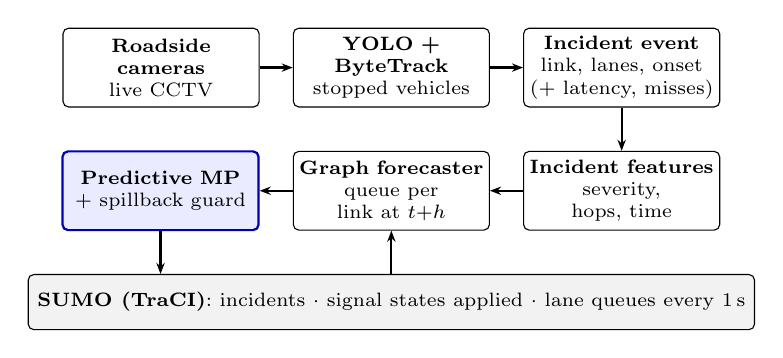
\begin{tikzpicture}[font=\scriptsize,
  box/.style={draw, rounded corners=2pt, align=center, text width=2.35cm, minimum height=1.0cm, inner sep=2pt},
  main/.style={box, draw=blue!70!black, fill=blue!8, thick},
  arr/.style={-{Stealth[length=4pt]}, thick}, node distance=0.45cm and 0.42cm]
\node[box] (cam) {\textbf{Roadside cameras}\\live CCTV};
\node[box, right=of cam] (det) {\textbf{YOLO + ByteTrack}\\stopped vehicles};
\node[box, right=of det] (evt) {\textbf{Incident event}\\link, lanes, onset\\(+ latency, misses)};
\node[box, below=0.55cm of evt] (pert) {\textbf{Incident features}\\severity, hops, time};
\node[box, left=of pert] (gnn) {\textbf{Graph forecaster}\\queue per link at $t{+}h$};
\node[main, left=of gnn] (ctl) {\textbf{Predictive MP}\\+ spillback guard};
\node[draw, rounded corners=2pt, fill=gray!10, align=center, minimum height=0.7cm, below=0.55cm of gnn, minimum width=8.2cm] (sumo) {\textbf{SUMO (TraCI)}: incidents $\cdot$ signal states applied $\cdot$ lane queues every 1\,s};
\draw[arr] (cam)--(det); \draw[arr] (det)--(evt); \draw[arr] (evt)--(pert); \draw[arr] (pert)--(gnn); \draw[arr] (gnn)--(ctl);
\draw[arr] (ctl.south)--(ctl.south |- sumo.north); \draw[arr] (sumo.north -| gnn.south)--(gnn.south);
\end{tikzpicture}
\caption{Closed-loop framework. In the control experiments the detection output is emulated with latency and missed detections.}
\label{fig:framework}
\end{figure}

\subsection{Incident Detection}
A COCO-pretrained YOLO model detects vehicles and ByteTrack assigns identities. A track is \emph{stopped} if its centre moves less than $v_{\text{stop}}$ box-heights per second over $T_{\text{stop}}$\,s; an alarm is confirmed when at least $n_{\min}$ tracks are stopped for $c$ consecutive frames. Parameters are tuned on the TADS training split; evaluating on TADS (966 accident segments, a 77.1\,GB frame archive) is left to future work, and its measured time-to-detect will replace the emulated latency. The protocol counts a segment as detected if an alarm falls between 2\,s before its labelled start and its end, counts alarms outside all segments (with a 10\,s margin) as false alarms, and reports precision, recall, F1, false alarms per hour, time-to-detect and frames per second. Because TADS provides gaze regions instead of boxes~\cite{xu2025sttad}, the detector is used without fine-tuning.

\subsection{Incident-Conditioned Graph Forecaster}
Links are nodes of a directed graph. Every 10\,s, link $i$ has features from its halting count $q_i(t)$ and its 30\,s and 60\,s changes, the summed queues of upstream and downstream neighbours (one-hop aggregation), and occupancy $q_i/\kappa_i$ ($\kappa_i$: storage capacity). Once an incident on link $k$ is \emph{known}, the blocked-lane fraction $s_k=n_k^{\text{blocked}}/n_k^{\text{lanes}}$ is added, masked by the hop distance of $i$ to $k$ (0--2), with elapsed time and interactions with $q_i$ and the upstream queue. One model shared by all links predicts $q_i(t+h)-q_i(t)$ for $h=120$\,s, so it transfers to unseen incident locations. We compare ridge regression with gradient-boosted trees~\cite{friedman2001gbm}.

\subsection{Predictive Max-Pressure with Spillback Guard}
Reactive MP~\cite{varaiya2013maxpressure} gives green to the phase maximising $P_p=\sum_{(l,m)\in p}(q_l-q_m)$ over movements from lane $l$ to lane $m$. The predictive controller adds the forecast change of each lane's link $e(l)$, spread over its $n_{e(l)}$ lanes:
\begin{equation}
\hat q_l=\max\!\Big(0,\,q_l+\tfrac{\hat q_{e(l)}(t{+}h)-q_{e(l)}(t)}{n_{e(l)}}\Big),\quad P_p=\!\!\sum_{(l,m)\in p}\!\!(\hat q_l-\hat q_m).
\end{equation}
\textbf{Spillback guard:} a movement is dropped when its outgoing link is forecast above $\theta=0.85$ of storage. Phases switch after a 10\,s minimum green, with 3\,s yellow and 60\,s maximum green. Algorithm~\ref{alg:loop} summarises one control step.

\begin{algorithm}[!htbp]
\caption{One step of the closed loop (every 1\,s)}
\label{alg:loop}
\begin{algorithmic}[1]
\State read lane queues $q_l$ from detectors
\If{an incident on link $k$ is reported (after latency $L$)}
  \State set incident features: $s_k$, hop distance to $k$, elapsed time
\EndIf
\If{$t \bmod 10\,\text{s} = 0$}
  \State build features for every link; forecast $\hat q_e(t{+}h)$ with the shared model
\EndIf
\For{each intersection $j$}
  \If{in yellow} \State count down; on expiry switch to the target phase
  \ElsIf{green time $\geq$ 10\,s}
    \State compute $\hat q_l$ (Eq.~1); drop movements whose outgoing link is forecast $>\theta$
    \State $p^\star \gets \arg\max_p P_p$
    \If{$P_{p^\star} > P_{\text{current}}$ \textbf{or} green time $\geq$ 60\,s} \State start 3\,s yellow towards $p^\star$ \EndIf
  \EndIf
\EndFor
\end{algorithmic}
\end{algorithm}

\subsection{Detection Emulation}
The incident becomes known to the controller after latency $L\in\{0,60,120,300\}$\,s, or never (``missed'').

\section{Experimental Setup}
\textbf{Network and demand.} A $4\times4$ signalised grid (SUMO 1.28), 200\,m two-lane links, two-phase signals. Random fringe-to-fringe trips plus an east--west arterial corridor: medium ($\approx$2{,}000 + 1{,}100\,veh/h) and high ($\approx$2{,}900 + 1{,}500\,veh/h) demand. Half of the vehicles reroute dynamically (period 60\,s). Runs last 3{,}000\,s.
\textbf{Incidents.} At $t=600$\,s, one or both lanes of the central corridor link are blocked for 1{,}200\,s. This location was not used in training: forecasters were trained on 60 runs with incidents on five other links and separate seeds. Each of the 4 test scenarios uses 8 seeds.
\textbf{Controllers.} Fixed-time (90\,s cycle), SUMO actuated (gap-out), reactive MP, and predictive MP with the linear forecaster, with the boosted forecaster without guard, and with boosted forecaster and guard (proposed). The boosted model was chosen on validation forecast error only, before any test control run.
Table~\ref{tab:param} lists the main settings.

\begin{table}[!htbp]
\centering
\caption{Simulation and model settings.}
\label{tab:param}
\setlength{\tabcolsep}{3pt}
\begin{tabular}{@{}ll@{}}
\toprule
Item & Setting \\
\midrule
Network & $4\times4$ grid, 200\,m links, 2 lanes, 13.9\,m/s \\
Signals & 2 green phases; min/max green 10/60\,s; yellow 3\,s \\
Demand (medium) & $\approx$2{,}000 random + 700/400 corridor veh/h \\
Demand (high) & $\approx$2{,}900 random + 1{,}000/500 corridor veh/h \\
Rerouting & 50\% of vehicles, period 60\,s \\
Incident & $t=600$\,s, 1{,}200\,s, 1 or 2 of 2 lanes blocked \\
Training data & 60 runs, 5 links, 6 seeds; 1.38\,M samples ($h=120$\,s) \\
Ridge model & 18 features, $\lambda=10$ \\
Boosted model & 200 trees, learning rate 0.1, 31 leaves; 300k samples \\
Model selection & validation seed held out; forecast error only \\
Test & unseen link, 2 demand $\times$ 2 blockage levels $\times$ 8 seeds \\
\bottomrule
\end{tabular}
\end{table}

\textbf{Metrics.} Average delay (time loss over all vehicles that entered), throughput, and $\Delta_{\text{shift}}=\sum_{i\in\mathcal{V}_{\text{far}}}(W_i^{\text{ctrl}}-W_i^{\text{MP}})$, where $W_i$ is halting time (veh$\cdot$h) on links at least two hops from the incident. Differences to reactive MP use the paired Wilcoxon test.

\section{Results}
\subsection{Forecast Accuracy (RQ1)}
Table~\ref{tab:fc} reports 2-minute queue forecasts on the 32 test runs. Over all links the boosted model gains only 4\% over persistence, since most queues barely change; near the incident it cuts error by 16.2\%. The linear model is worse than persistence, showing that incident effects are non-linear.

\begin{table}[!htbp]
\centering
\caption{MAE (vehicles) of 2-min link queue forecasts on test runs.}
\label{tab:fc}
\setlength{\tabcolsep}{3.5pt}
\begin{tabular}{@{}lcccc@{}}
\toprule
Links & Persistence & Linear & Boosted & Gain \\
\midrule
All (737{,}280 samples) & 0.472 & 0.489 & 0.453 & 4.0\% \\
$\leq$2 hops from incident (111{,}360) & 1.011 & 1.116 & 0.847 & 16.2\% \\
\bottomrule
\end{tabular}
\end{table}

Fig.~\ref{fig:ts} shows one test run (high demand, full closure). On the incident link and its upstream link, persistence lags every change by the 2-minute horizon, whereas the boosted forecast follows the onset and the clearance more closely; during the incident window its error is 3.3 vs.\ 5.4 vehicles on the incident link and 5.3 vs.\ 9.6 on the upstream link. On a diversion feeder two hops away, where queues are smaller and noisier, it is no better than persistence (3.5 vs.\ 3.3) and produces occasional spikes.

\begin{figure}[!htbp]
\centering
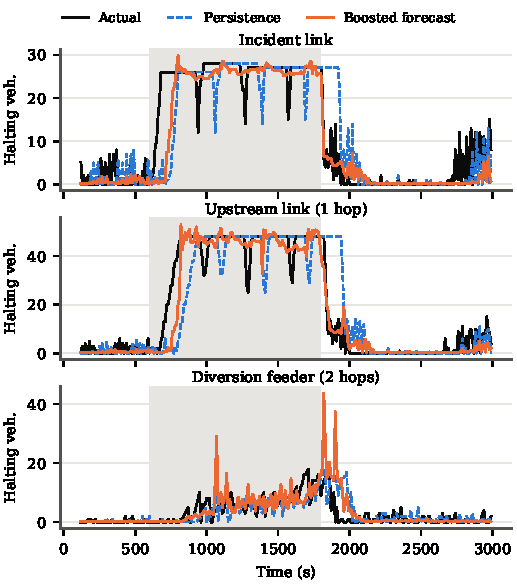
\includegraphics[width=\columnwidth]{figures/fig_timeseries.pdf}
\caption{Actual queue at $t{+}120$\,s, the persistence forecast and the boosted forecast for three links in one test run (high demand, full closure, seed 1). Shaded: incident active (600--1800\,s).}
\label{fig:ts}
\end{figure}

\subsection{Control Performance (RQ2)}

Table~\ref{tab:ctl} and Fig.~\ref{fig:delay} give three findings. \emph{First, better forecasts did not lower delay.} The proposed controller stayed within 1.2\,s/veh of reactive MP; the difference was not significant in three scenarios ($p\geq0.38$) and significantly worse by 1.2\,s/veh with high demand and one lane blocked ($p=0.008$). Under full closure it completed 40--55 fewer trips/h (medium: 2{,}793 vs.\ 2{,}847; high: 3{,}710 vs.\ 3{,}752), while actuated control completed the most (2{,}951 and 3{,}844). The linear-forecast variant was significantly worse in three scenarios, so a poor forecaster hurts more than a good one helps. \emph{Second, the guard was rarely active:} with one lane blocked no outgoing link was forecast above 85\% of storage, so guarded and unguarded results are identical. \emph{Third, actuated control was best} in all scenarios, 14.3\% (medium) and 15.5\% (high) below reactive MP under full closure. No predictive controller shifted congestion: $|\Delta_{\text{shift}}|\leq0.7$\,veh$\cdot$h with the boosted forecaster, whereas fixed-time added 17--30\,veh$\cdot$h of queuing on far links (Table~\ref{tab:shift}). Under full closure, every controller had 15--21 teleports per run (vehicles removed by SUMO after 300\,s of gridlock), showing that the closure saturates the corridor regardless of the signal policy.

\begin{table}[!htbp]
\centering
\caption{Average delay (s/veh, mean $\pm$ 95\% CI over 8 seeds). $^{\dagger}$: differs from reactive MP (Wilcoxon, $p<0.05$).}
\label{tab:ctl}
\footnotesize
\setlength{\tabcolsep}{2pt}
\begin{tabular}{@{}lcccc@{}}
\toprule
 & \multicolumn{2}{c}{Medium demand} & \multicolumn{2}{c}{High demand} \\
\cmidrule(lr){2-3}\cmidrule(l){4-5}
Controller & 1 lane & Closure & 1 lane & Closure \\
\midrule
Fixed-time & 62.5$\pm$0.7$^{\dagger}$ & 132.0$\pm$1.1$^{\dagger}$ & 79.1$\pm$1.9$^{\dagger}$ & 123.0$\pm$1.7$^{\dagger}$ \\
Actuated & \textbf{26.5}$\pm$0.2$^{\dagger}$ & \textbf{92.3}$\pm$1.2$^{\dagger}$ & \textbf{30.9}$\pm$0.4$^{\dagger}$ & \textbf{87.4}$\pm$2.8$^{\dagger}$ \\
Reactive MP & 34.3$\pm$0.4 & 107.7$\pm$2.1 & 42.2$\pm$0.4 & 103.4$\pm$2.2 \\
Pred.\ MP, linear & 36.1$\pm$0.7$^{\dagger}$ & 109.9$\pm$1.6$^{\dagger}$ & 43.1$\pm$0.8$^{\dagger}$ & 107.0$\pm$6.3 \\
Pred.\ MP, no guard & 34.7$\pm$0.6 & 108.2$\pm$2.0 & 43.4$\pm$0.9$^{\dagger}$ & 102.4$\pm$2.1 \\
Pred.\ MP + guard & 34.7$\pm$0.6 & 108.8$\pm$1.9 & 43.4$\pm$0.9$^{\dagger}$ & 102.9$\pm$2.7 \\
\bottomrule
\end{tabular}
\end{table}

\begin{table}[!htbp]
\centering
\caption{Congestion shift $\Delta_{\text{shift}}$ (veh$\cdot$h, vs.\ reactive MP; mean over 8 seeds).}
\label{tab:shift}
\setlength{\tabcolsep}{3pt}
\begin{tabular}{@{}lcccc@{}}
\toprule
 & \multicolumn{2}{c}{Medium} & \multicolumn{2}{c}{High} \\
\cmidrule(lr){2-3}\cmidrule(l){4-5}
Controller & 1 lane & Closure & 1 lane & Closure \\
\midrule
Fixed-time & $+16.8$ & $+17.5$ & $+29.6$ & $+20.3$ \\
Actuated & $-3.1$ & $-4.9$ & $-4.3$ & $-6.1$ \\
Pred.\ MP, linear & $+0.9$ & $+0.8$ & $+0.8$ & $+2.7$ \\
Pred.\ MP + guard & $+0.2$ & $+0.4$ & $+0.7$ & $-0.3$ \\
\bottomrule
\end{tabular}
\end{table}

\begin{figure}[!htbp]
\centering
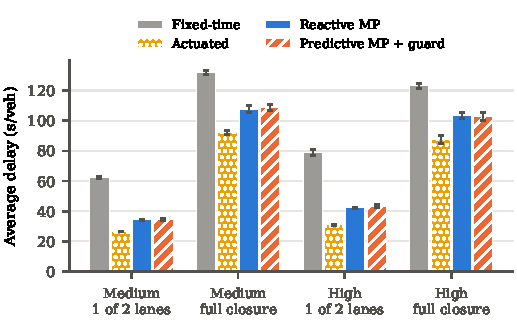
\includegraphics[width=\columnwidth]{figures/fig_delay_ieee.pdf}
\caption{Average delay per scenario (mean and 95\% CI, 8 seeds).}
\label{fig:delay}
\end{figure}

\subsection{Detection Latency and Misses (RQ3)}
Under full closure, latencies of 60--300\,s changed the proposed controller's delay by at most 1.5\,s/veh (medium: 108.8 to 110.3; high: 102.4 to 103.3\,s/veh). With the incident never reported, delay was 107.6 (medium) and 100.9\,s/veh (high), i.e., no worse. Here the incident features carried little information beyond the measured queues (Fig.~\ref{fig:lat}).

\begin{figure}[!htbp]
\centering
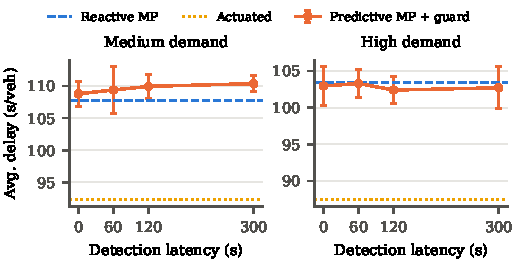
\includegraphics[width=\columnwidth]{figures/fig_latency_ieee.pdf}
\caption{Delay of the proposed controller versus detection latency under full closure (mean and 95\% CI), with reactive MP and actuated control as references.}
\label{fig:lat}
\end{figure}

\subsection{Unseen Incident Durations}
All training and main-test incidents lasted 1{,}200\,s. To test whether the forecaster had simply learned this duration, we repeated the full-closure tests with 600\,s and 1{,}800\,s incidents (8 seeds each, Table~\ref{tab:dur}). For the shorter incident the forecaster still beat persistence near the incident (13.5--21.0\% lower error), yet the predictive controller was significantly \emph{worse} than reactive MP (+5.4 and +7.9\,s/veh, $p=0.008$). For the longer incident the forecaster was 23--27\% \emph{worse} than persistence, confirming that it had partly learned the training duration through its elapsed-time feature, and the controller was not significantly different from reactive MP ($p\geq0.055$). Actuated control remained best in all cases.

\begin{table}[!htbp]
\centering
\caption{Full closure with unseen incident durations: delay (s/veh, mean $\pm$ 95\% CI, 8 seeds) and forecast-error change vs.\ persistence near the incident (negative = worse).}
\label{tab:dur}
\setlength{\tabcolsep}{2.6pt}
\begin{tabular}{@{}llcccc@{}}
\toprule
Duration & Demand & Actuated & Reactive MP & Pred.\ MP + guard & Forecast \\
\midrule
600\,s & Medium & 47.5 $\pm$ 0.6 & 62.6 $\pm$ 0.9 & 70.5 $\pm$ 2.8$^{\dagger}$ & +21.0\% \\
600\,s & High & 53.1 $\pm$ 1.2 & 82.1 $\pm$ 2.2 & 87.5 $\pm$ 2.3$^{\dagger}$ & +13.5\% \\
1{,}800\,s & Medium & 124.3 $\pm$ 5.8 & 132.7 $\pm$ 2.1 & 135.1 $\pm$ 1.8 & $-$22.6\% \\
1{,}800\,s & High & 112.9 $\pm$ 4.7 & 124.4 $\pm$ 2.0 & 123.0 $\pm$ 2.6 & $-$27.4\% \\
\bottomrule
\end{tabular}
\end{table}

\section{Discussion}
\textbf{Why forecasts did not help.} MP re-decides every second after a 10\,s minimum green, so it reacts to a growing queue within one or two decisions; a diverted platoon reaches the next junction within about one cycle, which the reactive policy already sees. Forecast errors on individual links add noise to the phase choice, which explains why the weaker linear forecaster hurt.
\textbf{Why actuated control won.} With two-phase plans, gap-out ends a green as soon as the approach empties, while halting-based MP reacts only once vehicles have stopped and pays fixed minimum-green and yellow costs. Reactive MP alone is therefore not a sufficient baseline for proactive control.
\textbf{When prediction should matter.} Prediction is more likely to pay off when actions need lead time (corridor offsets, route guidance~\cite{proactive2023divergent}), when the horizon matches incident-to-diversion travel times in larger networks, or when the controller optimises over a horizon (model-predictive control).
\textbf{Limitations.} One synthetic grid, two-phase signals, one test location and 50\% rerouting; the forecaster was trained on a single incident duration and does not generalise to longer incidents (Table~\ref{tab:dur}), so training must cover a realistic distribution of durations or use duration-free features; no empirical detection evaluation; a boosted-tree rather than a graph neural forecaster, although our results suggest forecast accuracy is not the bottleneck.

\section{Conclusion}
We built a closed loop from incident detection to incident-conditioned forecasting and predictive max-pressure control, and evaluated it on an unseen incident location with emulated detection latency. The forecaster reduced error near the incident by 16\%, but the controller matched reactive max-pressure, was worse for shorter unseen incidents, and a standard actuated controller performed best in every test. Incident-conditioned forecasts must also be trained across realistic incident durations to generalise. Future work will evaluate the detector on TADS, couple forecasts with controls that have real lead time, and test against strong actuated baselines on calibrated city networks.

\bibliographystyle{IEEEtran}
\bibliography{refs}
\end{document}
